% !TeX program = xelatex
\documentclass[a4paper,11pt]{article}

\usepackage[a4paper,margin=2.2cm]{geometry}
\usepackage{booktabs}
\usepackage{longtable}
\usepackage{array}
\usepackage{enumitem}
\usepackage{hyperref}
\usepackage{xcolor}
\usepackage{fancyvrb}
\usepackage{tikz}
\usepackage{pgfplots}

\usetikzlibrary{arrows.meta,positioning}
\pgfplotsset{compat=1.18}

\hypersetup{
  colorlinks=true,
  linkcolor=blue!55!black,
  urlcolor=blue!55!black
}

\setlist[itemize]{leftmargin=2em,itemsep=0.2em}
\setlist[enumerate]{leftmargin=2em,itemsep=0.2em}
\renewcommand{\arraystretch}{1.18}
\newcolumntype{L}[1]{>{\raggedright\arraybackslash}p{#1}}
\newcommand{\code}[1]{\texttt{#1}}
\newcommand{\artifact}[1]{\texttt{#1}}
\newcommand{\finding}[1]{\textbf{#1}}
\sloppy

\title{\bfseries Sakana Fugu Ultra \texorpdfstring{$\times$}{x} Codex CLI\\Long-Horizon Agent Behavior Report}
\author{Jason Chia-Sheng Lin\\\small Ph.D. Student, Institute of Biophotonics\\\small National Yang Ming Chiao Tung University}
\date{2026-05-14}

\begin{document}
\maketitle

\begin{abstract}
I analyze Sakana AI \code{fugu-ultra high} running a long Project II Phase II validation task inside OpenAI Codex CLI v0.130.0. My central conclusion is that Fugu Ultra did not fail because it lacked technical exploration ability; it failed as a long-horizon agent because it did not maintain enough state discipline. It explored repositories, Docker and IC setup, ELF properties, debugger evidence, coredumps, libc and gadget paths, and bounded sweeps. The failure point was state compression, negative-evidence preservation, convergence control, token budget management, and proof-boundary discipline. I compare the Fugu run with an Ubuntu GPT-5.5 handoff run and a Mac ARM64 GPT-5.5 completion attempt. I do not claim GPT-5.5 proved better exploit-solving ability. I claim that GPT-5.5 left a cleaner, more reproducible, more honest continuation state.
\end{abstract}

\tableofcontents
\newpage

\section{Introduction}

I write this report in the first person because I am making a defensible research judgment from observable logs, artifacts, token usage, git state, and validation boundaries. I separate verified facts from interpretation, and I state clearly which claims I do not make.

My core position is: \finding{I do not equate failure to solve the exploit with absence of model capability; I also do not equate large reasoning-token volume with task progress. I evaluate whether a long-horizon agent can convert exploration into durable state, negative evidence, stop rules, handoff artifacts, and an honest completion boundary.}

The effective Project II Phase II success condition is narrow:

\begin{Verbatim}[fontsize=\small]
The official IC Phase II workflow must produce /shared/success.txt.
\end{Verbatim}

I reject EC-side success-file creation, manual \artifact{/backdoor} execution, stale artifacts, coredump-only evidence, and scaffold-only checks as full-credit proof. This proof boundary is the foundation of the report.

\section{Evidence Sources}

\begin{longtable}{L{0.25\linewidth} L{0.38\linewidth} L{0.29\linewidth}}
\toprule
Evidence type & Copied log & How I use it\\
\midrule
Primary Fugu behavior log & Ubuntu Fugu Ultra Phase II validation source log in \path{source-logs/}. & I analyze token amplification, technical exploration, state drift, and unfinished official success.\\
GPT-5.5 handoff contrast & Ubuntu GPT-5.5 Phase II handoff source log in \path{source-logs/}. & I compare state compression and verified-fact handoff behavior.\\
GPT-5.5 Mac validation contrast & Mac ARM64 GPT-5.5 validation and publish source log in \path{source-logs/}. & I compare host recovery, deeper negative validation, artifact preservation, and git closeout.\\
\bottomrule
\end{longtable}

These logs are not a controlled A/B benchmark. I treat them as trajectory forensics: evidence for studying state discipline, context engineering, proof boundaries, negative evidence, and repository hygiene.

\section{Executive Finding}

My main conclusion is:

\begin{quote}
In this Codex CLI setting, \code{fugu-ultra} did not fail because it was incapable of technical exploration. It failed as a long-horizon agent because it did not maintain enough state discipline.
\end{quote}

Fugu Ultra performed real work: repository search, lab extraction, Docker/IC startup, ELF and gadget inspection, coredump validation, libc and one-gadget exploration, bounded sweeps, documentation updates, and static checks. The problem was not a lack of exploratory ability. The problem was that high-value findings were not compressed early enough into stable task state, failed-hypothesis ledgers, and proof-boundary gates.

The strongest evidence is the token/outcome contrast:

\begin{longtable}{L{0.32\linewidth} L{0.28\linewidth} L{0.30\linewidth}}
\toprule
Metric & Fugu value & Interpretation\\
\midrule
total tokens & 6,319,482 & Very high cost for an unfinished outcome.\\
input tokens & 6,136,936 & Active input pressure was extreme.\\
cached input & 23,226,988 & Long context was repeatedly reused.\\
output tokens & 182,546 & Large visible output did not become official completion.\\
reasoning tokens & 3,437,721 & Reasoning cost did not convert into the required proof artifact.\\
official success & not observed & No IC-side \artifact{/shared/success.txt}.\\
\bottomrule
\end{longtable}

\section{Three-Run Comparison}

\begin{longtable}{L{0.25\linewidth} L{0.22\linewidth} L{0.22\linewidth} L{0.23\linewidth}}
\toprule
Dimension & Ubuntu / Fugu Ultra & Ubuntu / GPT-5.5 handoff & Mac ARM64 / GPT-5.5 completion\\
\midrule
Main task & Direct Phase II completion & Handoff generation & Completion attempt + environment repair\\
Host friction & Low & Low & High\\
Technical exploration & High & Medium-low & High\\
State compression & Low & Very high & High\\
Negative evidence preservation & Medium-low & High & Very high\\
Honest completion boundary & Medium & High & Very high\\
Continuation readiness & Medium-low & Very high & Very high\\
Official \artifact{/shared/success.txt} & No & No & No\\
Total tokens & 6,319,482 & not shown & 1,098,226\\
Reasoning tokens & 3,437,721 & not shown & 52,062\\
Closeout state & Local modifications / incomplete closure & Handoff artifact & Commit \code{ab319c0}, pushed to main, clean worktree\\
\bottomrule
\end{longtable}

My interpretation is direct: Fugu Ultra explored deeply, but it did not convert exploration into a stable decision system quickly enough. GPT-5.5 did not solve the exploit either, but it produced a cleaner engineering state.

\section{Mac ARM64 Run: Environment Repair as Evidence}

The Mac run strengthens my conclusion because it was a harder host environment. The log verifies MacBook-Air, macOS, ARM64, and \code{ARM64\_T8112}. I therefore use ``Mac Air ARM64 host'' as the rigorous phrasing; I do not treat ``M1'' as log-verified hardware identity inside the report.

\begin{figure}[htbp]
\centering
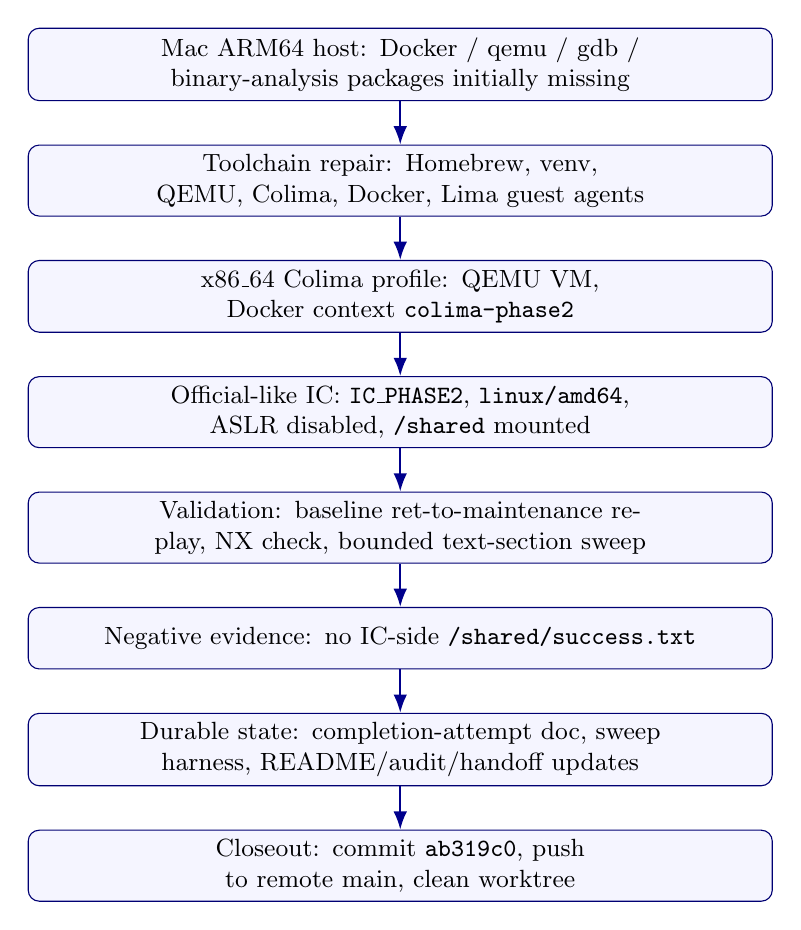
\begin{tikzpicture}[
  node distance=0.55cm,
  every node/.style={font=\small},
  box/.style={draw=blue!45!black, rounded corners, align=center, text width=0.76\linewidth, minimum height=0.78cm, fill=blue!4},
  arrow/.style={-Latex, thick, draw=blue!55!black}
]
\node[box] (a) {Mac ARM64 host: Docker / qemu / gdb / binary-analysis packages initially missing};
\node[box, below=of a] (b) {Toolchain repair: Homebrew, venv, QEMU, Colima, Docker, Lima guest agents};
\node[box, below=of b] (c) {x86\_64 Colima profile: QEMU VM, Docker context \code{colima-phase2}};
\node[box, below=of c] (d) {Official-like IC: \artifact{IC\_PHASE2}, \code{linux/amd64}, ASLR disabled, \artifact{/shared} mounted};
\node[box, below=of d] (e) {Validation: baseline ret-to-maintenance replay, NX check, bounded text-section sweep};
\node[box, below=of e] (f) {Negative evidence: no IC-side \artifact{/shared/success.txt}};
\node[box, below=of f] (g) {Durable state: completion-attempt doc, sweep harness, README/audit/handoff updates};
\node[box, below=of g] (h) {Closeout: commit \code{ab319c0}, push to remote main, clean worktree};
\draw[arrow] (a) -- (b);
\draw[arrow] (b) -- (c);
\draw[arrow] (c) -- (d);
\draw[arrow] (d) -- (e);
\draw[arrow] (e) -- (f);
\draw[arrow] (f) -- (g);
\draw[arrow] (g) -- (h);
\end{tikzpicture}
\caption{Mac ARM64 run as environment repair plus validation-state compression.}
\end{figure}

I consider this a meaningful agent-behavior result. GPT-5.5 turned host friction into a reproducible validation path instead of treating the missing environment as either success or a terminal blocker.

\section{Token and Reasoning Cost}

I chart only the two completion/validation runs with complete visible token usage. The Ubuntu GPT-5.5 handoff log did not expose token usage, so I exclude it from the numeric chart.

\begin{figure}[htbp]
\centering
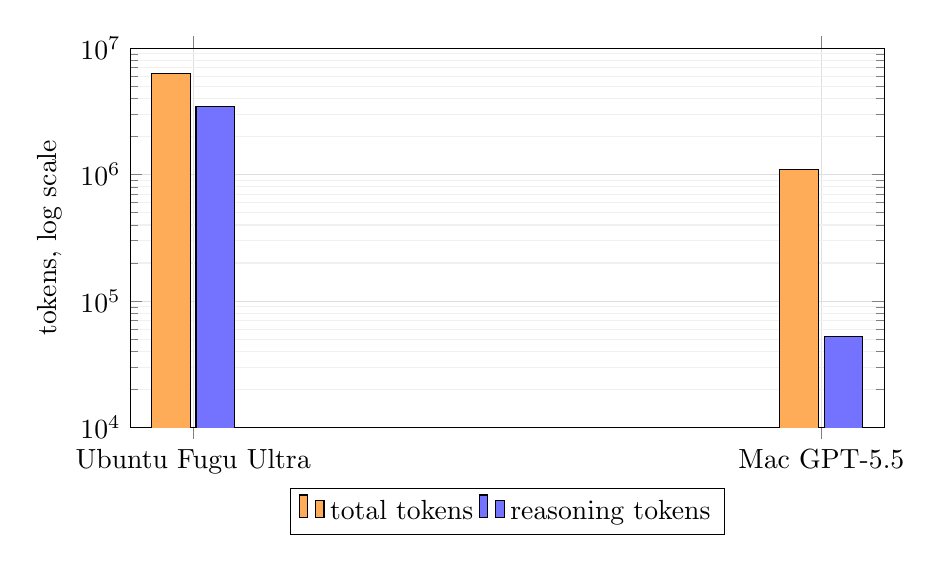
\begin{tikzpicture}
\begin{axis}[
  ybar,
  bar width=14pt,
  width=0.92\linewidth,
  height=6.4cm,
  ymode=log,
  ymin=10000,
  ymax=10000000,
  ylabel={tokens, log scale},
  symbolic x coords={Fugu,Mac},
  xtick=data,
  xticklabels={Ubuntu Fugu Ultra,Mac GPT-5.5},
  xticklabel style={align=center},
  legend style={at={(0.5,-0.16)},anchor=north,legend columns=2},
  grid=both,
  major grid style={draw=gray!25},
  minor grid style={draw=gray!12}
]
\addplot[fill=orange!65] coordinates {(Fugu,6319482) (Mac,1098226)};
\addplot[fill=blue!55] coordinates {(Fugu,3437721) (Mac,52062)};
\legend{total tokens,reasoning tokens}
\end{axis}
\end{tikzpicture}
\caption{Token cost comparison for the two runs with complete visible token usage.}
\end{figure}

\begin{longtable}{L{0.22\linewidth} L{0.20\linewidth} L{0.20\linewidth} L{0.30\linewidth}}
\toprule
Metric & Ubuntu Fugu Ultra & Mac GPT-5.5 & My interpretation\\
\midrule
Total tokens & 6,319,482 & 1,098,226 & Fugu used about 5.75x more total tokens.\\
Reasoning tokens & 3,437,721 & 52,062 & Fugu used about 66x more reasoning tokens.\\
Cached input & 23,226,988 & 28,131,328 & High cached context alone did not cause reasoning collapse.\\
Reasoning / total & 54.4\% & 4.7\% & Fugu concentrated cost in active reasoning.\\
Reasoning / output & 18.8:1 & 0.48:1 & Fugu converted reasoning into artifacts less efficiently.\\
\bottomrule
\end{longtable}

This is not a fully fair model benchmark because the Mac run had a prior handoff. Still, I find the behavior difference important: Fugu's reasoning expanded without closure, while GPT-5.5 kept reasoning more tightly coupled to decisions and artifacts.

\section{Technical Negative Evidence}

The Mac run did not solve Phase II. Its value is that it made several plausible paths explicitly non-repeatable:

\begin{longtable}{L{0.25\linewidth} L{0.31\linewidth} L{0.35\linewidth}}
\toprule
Path tested & Result & Why I consider it useful\\
\midrule
Current ret-to-\code{maintenance\_task+5} candidate & \code{success\_exists=no}; no \artifact{/shared/success.txt}. & The candidate remains non-success; argument control is still unresolved.\\
Direct stack shellcode & Reached stack address but faulted under NX. & Stack-resident shellcode is excluded in the live runtime.\\
One-shot text-section partial return & \code{0x401000..0x401a20}, four prefixes, 10,328 candidates, no success. & The next agent should not rerun the same blind landing-point sweep.\\
Manual \artifact{/backdoor} & Sanity check only. & It is not official proof.\\
Colima/QEMU IC setup & Reproducible \code{x86\_64 linux/amd64} path. & Future runs should reuse this path rather than rebuilding the environment from scratch.\\
\bottomrule
\end{longtable}

My current technical conclusion is:

\begin{Verbatim}[fontsize=\small]
The core blocker is no longer "we have not confirmed overflow,"
"we have not confirmed the success condition," or
"we have not reproduced an official-like IC runtime."

The core blocker is:
how to obtain reliable pivot and first-argument control under
C-string / NUL-byte constraints.
\end{Verbatim}

\section{Behavior Scoring}

These scores describe behavior profiles, not absolute model intelligence.

\begin{longtable}{L{0.30\linewidth} L{0.18\linewidth} L{0.22\linewidth} L{0.22\linewidth}}
\toprule
Evaluation dimension & Fugu Ubuntu & GPT-5.5 Ubuntu handoff & GPT-5.5 Mac ARM64 completion\\
\midrule
Task understanding & 3.5/5 & 5/5 & 5/5\\
Environment understanding & 4/5 & 4/5 & 5/5\\
Environment repair & 3/5 & N/A & 5/5\\
Technical exploration & 4.5/5 & 3/5 & 4/5\\
Dynamic validation & 3/5 & 2/5 & 4.5/5\\
State compression & 1.5/5 & 5/5 & 4.5/5\\
Negative evidence quality & 2/5 & 3/5 & 5/5\\
Token efficiency & 1/5 & High, but no token count & 3.5/5\\
Completion-boundary honesty & 3/5 & 5/5 & 5/5\\
Repository hygiene & 2.5/5 & 4/5 & 5/5\\
Final exploit success & 0/5 & N/A & 0/5\\
\bottomrule
\end{longtable}

My conclusion from this table is not that GPT-5.5 solved the exploit. It did not. My conclusion is that GPT-5.5 managed the unsolved state more professionally.

\section{Beyond Pass/Fail: Evaluating the Quality of Unfinished Agent States}

Traditional agent benchmarks often over-emphasize binary completion: a run either solves the task or it does not. I consider that insufficient for long-horizon agent systems. Long tasks frequently end in partially solved states: environment-recovery states, validated negative evidence, handoff artifacts, constrained hypothesis spaces, or unfinished debugging trajectories. These states are not equivalent.

My central claim in this section is:

\begin{quote}
A long-horizon agent should not only be evaluated by whether it reaches the goal, but also by whether it leaves the search space in a lower-entropy state.
\end{quote}

\subsection{Unfinished State and Failure Quality}

I define an \finding{unfinished agent state} as the set of artifacts, verified facts, negative evidence, environment state, reasoning compression, and continuation constraints left behind after a non-completed run.

I define \finding{failure quality} as the degree to which an unsuccessful run reduces uncertainty for future runs. A high-quality failure narrows the hypothesis space, eliminates dead ends, preserves evidence, improves reproducibility, and increases continuation readiness. A low-quality failure repeats exploration, increases context entropy, loses evidence provenance, or leaves ambiguous completion state.

\begin{longtable}{L{0.30\linewidth} L{0.30\linewidth} L{0.30\linewidth}}
\toprule
Run & Binary outcome & Unfinished-state quality\\
\midrule
Ubuntu Fugu Ultra & Unfinished & High exploration, but low convergence and high active-context entropy.\\
Ubuntu GPT-5.5 handoff & Unfinished & High state compression through explicit FACT / THEORY / REPORTED-UNVERIFIED separation.\\
Mac ARM64 GPT-5.5 & Unfinished & High negative-evidence preservation, environment reconstruction, reproducible harnessing, and clean repo closeout.\\
\bottomrule
\end{longtable}

None of the three runs solved the exploit. Yet the engineering value of their unfinished states was not equal. This is the central evaluation signal that a binary pass/fail benchmark would discard.

\subsection{Capability Failure Versus Harness Governance Failure}

I do not interpret the Fugu trajectory as a pure capability failure. It is also a harness-governance failure. The run lacked hard budget gates, no-new-evidence stop rules, forced checkpointing, duplicate-command detection, and proof-boundary gates strong enough to convert exploration into durable state.

\begin{quote}
This is not only a model problem. It is a harness governance problem.
\end{quote}

In this case, a stronger governance layer would have required periodic external state compression, a failed-hypothesis ledger, explicit proof-boundary checks before declaring progress, and a rule that extended exploration must earn new evidence rather than merely produce more trace.

\subsection{Entropy Reduction and Marginal Evidence Yield}

In this report, entropy means the uncertainty remaining about the environment, exploit surface, failed hypotheses, valid proof boundaries, and next-step action space. A useful long-horizon agent reduces that entropy over time. A drifting agent may continue spending tokens while reducing little additional uncertainty.

\begin{figure}[htbp]
\centering
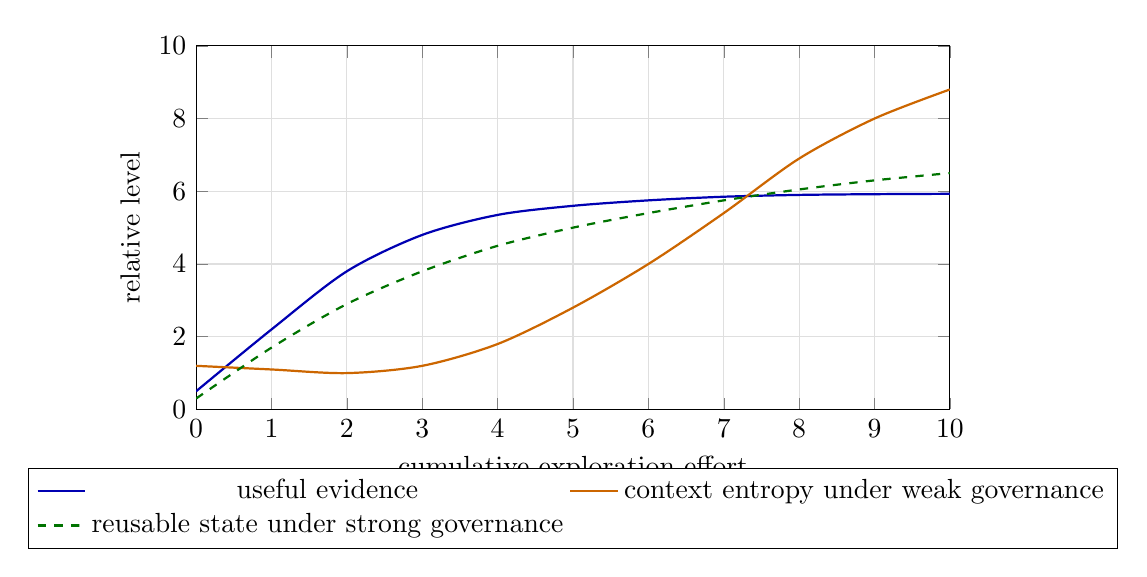
\begin{tikzpicture}
\begin{axis}[
  width=0.92\linewidth,
  height=6.2cm,
  xmin=0,
  xmax=10,
  ymin=0,
  ymax=10,
  xlabel={cumulative exploration effort},
  ylabel={relative level},
  legend style={at={(0.5,-0.16)},anchor=north,legend columns=2},
  grid=both,
  major grid style={draw=gray!25}
]
\addplot[blue!70!black, thick, smooth] coordinates {(0,0.5) (1,2.2) (2,3.8) (3,4.8) (4,5.35) (5,5.6) (6,5.75) (7,5.85) (8,5.9) (9,5.92) (10,5.93)};
\addplot[orange!80!black, thick, smooth] coordinates {(0,1.2) (1,1.1) (2,1.0) (3,1.2) (4,1.8) (5,2.8) (6,4.0) (7,5.4) (8,6.9) (9,8.0) (10,8.8)};
\addplot[green!45!black, thick, dashed, smooth] coordinates {(0,0.3) (1,1.7) (2,2.9) (3,3.8) (4,4.5) (5,5.0) (6,5.4) (7,5.75) (8,6.05) (9,6.3) (10,6.5)};
\legend{useful evidence, context entropy under weak governance, reusable state under strong governance}
\end{axis}
\end{tikzpicture}
\caption{Conceptual entropy curve: after marginal evidence yield declines, weak governance lets context entropy dominate; strong governance externalizes state before drift compounds.}
\end{figure}

The Fugu run reduced uncertainty about ELF structure, coredump behavior, libc mappings, runtime mitigations, and plausible gadget paths. However, this reduction was partially offset by repeated exploration, weak state compression, and token amplification. GPT-5.5 reduced entropy more efficiently by compressing verified facts, preserving negative evidence, and externalizing continuation state into repository artifacts.

\subsection{Handoff Artifact Quality Rubric}

To make this evaluation repeatable, I propose a 100-point handoff artifact quality rubric:

\begin{longtable}{L{0.36\linewidth} L{0.12\linewidth} L{0.42\linewidth}}
\toprule
Dimension & Points & What I would score\\
\midrule
Objective clarity & 10 & Is the final success condition explicit and testable?\\
Proof boundary & 15 & Does the artifact distinguish official proof from invalid or partial proof?\\
Verified facts & 15 & Are confirmed facts separated from speculation and stale reports?\\
Failed paths & 15 & Are dead ends recorded with enough detail to prevent reruns?\\
Negative evidence & 15 & Are failed tests reproducible, bounded, and tied to observable outcomes?\\
Reproducible commands & 10 & Can the next agent rebuild the environment or rerun checks?\\
Next-action contract & 10 & Does the artifact narrow the next hypothesis or decision gate?\\
Repository hygiene & 10 & Are files organized, committed, and easy to locate?\\
\bottomrule
\end{longtable}

This rubric evaluates what remains after the run, not only what happened during the run. It makes continuation readiness a first-class metric.

\subsection{Evaluation Dimensions Beyond Binary Completion}

\begin{longtable}{L{0.32\linewidth} L{0.58\linewidth}}
\toprule
Metric & Description\\
\midrule
Completion rate & Whether the final task was solved.\\
False-completion rate & Whether the agent incorrectly claimed success.\\
State compression quality & How well verified state was externalized into durable artifacts.\\
Negative-evidence preservation & Whether failed paths were recorded in a reusable form.\\
Continuation readiness & How easily a next agent can resume without rediscovery.\\
Entropy reduction & How much uncertainty was removed from the environment, hypothesis space, and proof boundary.\\
Marginal evidence yield & Useful evidence gained per additional token, tool call, or time block.\\
Drift resistance & Ability to avoid recursive rediscovery and generic status regression.\\
Proof-boundary discipline & Separation of official proof, sanity checks, partial progress, and speculation.\\
Repo hygiene & Clarity of artifact organization, commits, and handoff paths.\\
\bottomrule
\end{longtable}

This framework matters because future agents will operate in scientific workflows, software engineering, cybersecurity labs, autonomous debugging, and infrastructure recovery. In these domains, an agent that fails honestly and leaves reusable state may be more valuable than an agent that produces an unverifiable success claim.

\section{Claims I Make and Claims I Reject}

I conclude:

\begin{itemize}
  \item Fugu Ultra showed real technical exploration ability.
  \item Fugu Ultra's main failure mode was long-horizon state discipline: token amplification, memory fragmentation, delayed compression, and weak convergence control.
  \item GPT-5.5 showed stronger context engineering in the handoff run.
  \item GPT-5.5 showed stronger host-environment recovery and negative-evidence preservation in the Mac run.
  \item The repository itself should be treated as the durable memory system for long-running agents.
\end{itemize}

I do not conclude:

\begin{itemize}
  \item I do not conclude that GPT-5.5 is proven to be better at solving this exploit.
  \item I do not conclude that Fugu Ultra lacks technical ability.
  \item I do not conclude that Codex CLI hierarchical memory alone caused the failure.
  \item I do not conclude that the Mac run achieved full-credit Project II completion.
\end{itemize}

The sharper claim is:

\begin{quote}
Fugu Ultra lost control of long-horizon state; GPT-5.5 preserved state better. The decisive difference in these logs is not solved-vs-unsolved exploit outcome, but the quality of the unfinished state left behind.
\end{quote}

\section{Next Fair Experiment Matrix}

\begin{longtable}{L{0.08\linewidth} L{0.16\linewidth} L{0.18\linewidth} L{0.28\linewidth} L{0.22\linewidth}}
\toprule
Group & Host & Model & Starting point & Purpose\\
\midrule
A & Ubuntu 24 & Fugu Ultra & \artifact{HANDOFF\_PHASE2.md} + Mac negative evidence & Test whether external memory reduces Fugu drift.\\
B & Ubuntu 24 & GPT-5.5 & Mac 2026-05-14 artifacts & Test whether GPT can exploit the new negative evidence.\\
C & Mac ARM64 & Fugu Ultra & Same handoff + existing Colima runbook & Test Fugu host recovery and state discipline.\\
D & Mac ARM64 & GPT-5.5 & Already-built Colima IC & Isolate exploit reasoning from environment bootstrap.\\
\bottomrule
\end{longtable}

The key metrics should be official success rate, false-completion rate, tokens per useful evidence item, duplicate-command rate, failed-hypothesis retry rate, no-new-evidence streak, artifact quality, repo hygiene, and time-to-official-validation.

\section{Final Conclusion}

My final conclusion is:

\begin{quote}
Fugu Ultra in the Ubuntu native run showed strong exploration but weak convergence. GPT-5.5 in the Ubuntu handoff run performed state compression. GPT-5.5 in the Mac ARM64 run, despite a harder host environment, built an x86\_64 Colima validation path, produced deeper negative evidence, preserved a reproducible sweep harness, updated the repository, and pushed a clean commit.
\end{quote}

I keep the boundary explicit:

\begin{quote}
GPT-5.5 did not complete Project II full-credit success. It completed a cleaner, more reproducible, more honest engineering-validation loop.
\end{quote}

That distinction is the research value of this packet. In an agent-system evaluation, the strongest evidence is not who solved the exploit. No run solved it. The strongest evidence is what each agent left behind when it failed:

\begin{Verbatim}[fontsize=\small]
Fugu Ultra left a high-token, low-convergence long trace.
GPT-5.5 left durable docs, a harness, a pushed commit, and negative evidence.
\end{Verbatim}

That is the difference I would carry into the next agent benchmark design.

\end{document}
